\subsection{Zero absoluto: Determinação do zero absoluto utilizando um termômetro a
gás}

A terceira prática tem como objetivo determinar a temperatura do zero absoluto. Para isso, será utilizado o termômetro a gás, a volume constante, que consiste em um bulbo de vidro contendo hélio, que é então ligado a um barômetro do tipo Torricelli. Esse sistema pode ser observado na representação esquemática a seguir:

\begin{figure}[H]
  \centering
  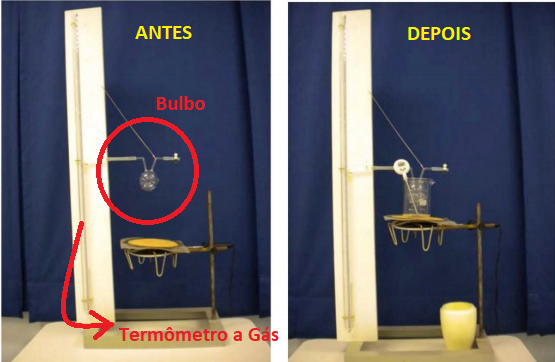
\includegraphics[scale=0.9]{images/Termômetro a Gás.png}
  \caption{Representação do Termômetro a Gás.}
\end{figure}

O termômetro é formado por um tubo em “U” contendo mercúrio em seu interior e com um dos braços lacrados para que a pressão em seu interior seja zero. No outro braço é colocado um balão de vidro contendo gás hélio a uma pressão próxima da pressão atmosférica. Para a leitura da pressão nesse barômetro, basta observar que a pressão exercida pelo gás Hélio em um ponto A do braço é exatamente igual à pressão exercida pela coluna de mercúrio sobre o ponto B do outro braço, a qual pode ser obtida diretamente pela sua altura h em cmHg (centímetro de mercúrio).

\begin{figure}[H]
  \centering
  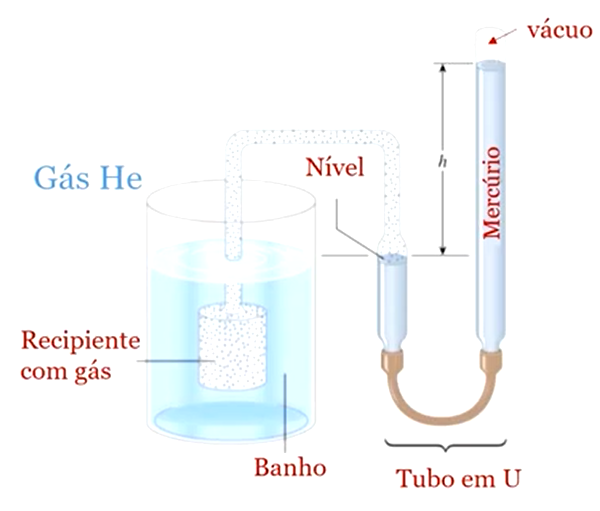
\includegraphics[scale=0.75]{images/Termômetro a Gás esquemático.png}
  \caption{Esquemático dos elementos que compõem o termômetro a gás.}
\end{figure}

O experimento consiste, então, em medir a pressão do gás para diversas temperaturas obtidas na seguinte ordem:

\begin{enumerate}
    \item Bulbo mergulhado em água à temperatura ambiente;
    \item Bulbo mergulhado em gelo em fusão;
    \item Bulbo mergulhado em nitrogênio líquido;
    \item Bulbo mergulhado em água em ebulição.
\end{enumerate}

Após isso, será construído um gráfico da pressão (medida em cmHg) em função da temperatura (medida em ºC). A partir do método dos mínimos quadrados, será determinado o coeficiente de dilatação do gases ideais a volume constante ($\beta$) e o valor de $P_0$. Essa relação pode ser comprovada a partir de uma equação em que ao aumentar a temperatura de um gás, mantido volume constante, a pressão varia linearmente com a temperatura. Se a temperatura inicial do gás é 0ºC e sua pressão inicial é $P_0$, a pressão P(T), à temperatura T(ºC), será dada por:

\[ P(T) = P_0 \cdot (\beta \cdot T + 1) = P_0 \cdot \beta \cdot T + P_0 \]\

Nesse caso, $P_0$ corresponde ao coeficiente linear da reta e o valor do coeficiente $\beta$ pode ser relacionado diretamente ao coeficiente angular, que nesse caso será igual a $\beta P_0$.\\

Com os valores de $\beta$ e $P_0$, escreve-se a equação que descreve o comportamento da variação da pressão do gás em função da temperatura. Utilizando essa equação, será construído uma reta sobre os pontos experimentais e a partir da extrapolação desta reta será determinado a temperatura zero absoluto. Essa situação corresponde à menor temperatura que se pode alcançar fisicamente.\\